\documentclass[a4paper,12pt, notitlepage]{article}
\usepackage[margin=2.5cm]{geometry}
\usepackage{listings}
\usepackage[parfill]{parskip}
\setlength{\parskip}{\baselineskip}%
\setlength{\parindent}{0pt}%
\usepackage{amsmath}
\usepackage{amssymb}
\usepackage{graphicx}
\usepackage[justification=centering]{caption}
\usepackage{epstopdf}
\usepackage[usenames, dvipsnames]{color}
\usepackage{chngcntr}
\usepackage{titling}
%\counterwithout{footnote}{chapter}
\usepackage{float}
%\renewcommand\theContinuedFloat{\alph{ContinuedFloat}}
\newcommand\tab[1][0.05cm]{\hspace*{#1}}

\title{Numerical Assignment}
\author{Mariana Clare}
\date{\today}

\begin{document}
	
\maketitle
\thispagestyle{empty}
\section{Defining the Shallow Water Equations}
The shallow water equations are
\begin{equation}\label{momentumsw}
\frac{\partial \mathbf{u}}{\partial t} + \mathbf{u}\cdot\nabla\mathbf{u} = - 2\Omega \times\mathbf{u} - g\nabla (h + h_{0})
\end{equation}
\begin{equation}\label{masssw}
\frac{\partial h}{\partial t} + \mathbf{u}\cdot\nabla h = - h \nabla \cdot \mathbf{u}
\end{equation}
where $\mathbf{u}$ is the velocity of the flow, $\Omega$ is the angular velocity of the rotating frame of reference, $g$ is the gravitational acceleration constant, $h$ is the depth of the fluid and $h_{0}$ represents the underlying shape that the fluid is flowing over (as defined in \cite{MPE textbook}).

The first equation (\ref{momentumsw}) represents the conservation of momentum and the second equation (\ref{masssw}) represents the conservation of mass.

In order to solve these equations numerically, we first linearise them about the state $u = 0$ and $h = H$ ie.
\begin{eqnarray}\nonumber
\mathbf{u} =  & \mathbf{\hat{u}}
 \\   \nonumber
h = &  H + \hat{h} .
\end{eqnarray}
where $H$ is the average fluid depth. If we further assume that $h_{0}$ is constant, this gives
\begin{equation}
\frac{\partial \mathbf{\hat{u}}}{\partial t} = 2 \Omega \times \mathbf{\hat{u}} - g \nabla \hat{h}
\end{equation}
\begin{equation}
\frac{\partial \hat{h}}{\partial t} = - H \nabla \cdot \mathbf{\hat{u}}
\end{equation}

These equations can be simplified further by assuming that the frame is not rotating and taking the one-dimensional form. Dropping the $\hat{}$ notation this gives
\begin{equation}\label{linearisedsw1}
\frac{\partial u}{\partial t} = - g \frac{\partial h}{\partial x}
\end{equation}
\begin{equation}\label{linearisedsw2}
\frac{\partial h}{\partial t} = - H \frac{\partial u}{\partial x}.
\end{equation}
This report will seek to solve these one-dimensional lineriased shallow water equations numerically. Note that throughout this report we assume for simplicity that $u$ and $h$ have periodic boundary conditions.

\section{Numerical Methods}\label{numericalmethodssection}

\subsection {Co-located Explicit}
The first numerical method we use to attempt to solve (\ref{linearisedsw1}) and (\ref{linearisedsw2}) is a simple co-located forward-backward in time and centred in space scheme. As in \cite{MPE textbook}, we consider the scheme to be forward in $u$ and backward in $h$. Co-located means we define the velocity and the height at the same location on the meshgrid. Co-located schemes are also referred to as A-grid or unstaggered schemes.

This scheme can be written as 
\begin{equation} \label{FTCSAgrid}
\frac{u_{j}^{(n+1)} - u_{j}^{(n)}}{\Delta t} = -g \frac{h_{j+1}^{(n)} - h_{j-1}^{(n)}}{2\Delta x}
\end{equation}
\begin{equation}\label{BTCSAgrid}
\frac{h_{j}^{(n+1)} - h_{j}^{(n)}}{\Delta t} = -H \frac{u_{j+1}^{(n+1)} - u_{j-1}^{(n+1)}}{2\Delta x}
\end{equation}
where $h_{j}^{(n)} = h(x_{j}, t^{(n)})$, $u_{j}^{(n)} = h(u_{j}, t^{(n)})$, $x_{j} = j\Delta x$ and $t^{(n)} = n\Delta t$. 

We can determine the order of accuracy of this scheme, by using Taylor series. We note the following Taylor series expansions:

\begin{equation}\label{ujn+1}
u_{j}^{(n+ 1)} = u_{j}^{(n)} + \Delta t \frac{\partial u_{j}^{(n)}}{\partial t} + \frac{(\Delta t)^{2}}{2}\frac{\partial^{2} u_{j}^{(n)}}{\partial t^{2}} + O((\Delta t)^{3})
\end{equation}
\begin{equation}\label{hj+-1n}
h_{j \pm 1}^{(n)} = h_{j}^{(n)} \pm \Delta x  \frac{\partial h_{j}^{(n)}}{\partial x} + \frac{(\Delta x)^{2}}{2}\frac{\partial^{2} h_{j}^{(n)}}{\partial x^{2}} \pm \frac{(\Delta x)^{3}}{6}\frac{\partial^{3} h_{j}^{(n)}}{\partial x^{3}} + O((\Delta x)^{4})
\end{equation}

Substuting these expansions into the scheme (\ref{FTCSAgrid}), we find that 

\begin{equation}
\frac{\partial u_{j}^{(n)}}{\partial t} + O(\Delta t) =  -g \frac{\partial h_{j}^{(n)}}{\partial x} + O((\Delta x)^{2})
\end{equation} 
and therefore the scheme is first order accurate in time and second order accurate in space. (Note the same order of accuracy is obtained by performing the same analysis with equation (\ref{BTCSAgrid})).

In order to find when this scheme is stable, we use a Von-neumann stability analysis. As in \cite{MPE textbook}, we assume that $u$ and $h$ have wave-like solutions with an amplification factor $A$ and wavenumber $k$:
\begin{equation} \label{wavelikeu}
u  =  \mathbb{U}  A^{n} e^{ikj\Delta x}
\end{equation}
\begin{equation} \label{wavelikeh}
h  =  \mathbb{H} A^{n} e^{ikj\Delta x}
\end{equation}
for constant $\mathbb{U}$ and $\mathbb{H}$.

Further if we define the courant number 
\begin{equation}\label{courantnumber}
c = \frac{\sqrt{gH}\Delta t}{\Delta x}
\end{equation}

then substituting these solutions into (\ref{FTCSAgrid}) and (\ref{BTCSAgrid}) gives
\begin{equation}
A = 1 - \frac{c^{2}}{2} \sin^{2}(k\Delta x) \pm \frac{ic}{2}\sin(k\Delta x)\sqrt{4 - c^{2}\sin^{2}k\Delta x}.
\end{equation} 
 
Hence as found in \cite{MPE textbook}, when $\lvert c \rvert \leq 2$, $\lvert A \rvert^{2} = 1$ and the scheme is stable, but when $\lvert c \rvert > 2$, the scheme is unstable.
 
We can also find the dispersion relation, because the frequency of the numerical method is 
\begin{equation} \label{frequency}
\omega = \pm \frac{1}{\Delta t} \arctan\bigg(\frac{Im(A)}{Re(A)}\bigg)
\end{equation}
Using the result from \cite{MPE textbook}, 
\begin{equation}
\omega_{n}\Delta x = \pm \frac{2}{c} \sin^{-1} \bigg(\frac{c}{2}\sin(k\Delta x)\bigg)
\end{equation}
assuming $\sqrt{gH} = 1$. The positive branch of this dispersion relation is plotted in Figure \ref{dispersionfigure} and compared with the dispersion relation of the analytical solution. (The dispersion relation of the analytical solution $\omega = k\sqrt{gH}$ is found by substituting the wave-like solutions (\ref{wavelikeu}) and (\ref{wavelikeh}) into (\ref{linearisedsw1}) and (\ref{linearisedsw2})). This shows that the analytic solution and numerical solution do not propagate at the same rate. The numerical solution disperses too slowly and in fact for $k = \pi$, the wave is stationary.

\subsection{Co-located Implicit}
We would like to have a method that was stable for all courant numbers. Therefore another method we can use is an implicit method on a co-located grid. As in \cite{MPE textbook}, we will consider the backward in time for both $u$ and $h$ and centred in space co-located scheme:
\begin{equation} \label{FTimplicitAgrid1}
\frac{u_{j}^{(n+1)} - u_{j}^{(n)}}{\Delta t} = -g \frac{h_{j+1}^{(n+1)} - h_{j-1}^{(n+1)}}{2\Delta x}
\end{equation}
\begin{equation}\label{FTimplicitAgrid2}
\frac{h_{j}^{(n+1)} - h_{j}^{(n)}}{\Delta t} = -H \frac{u_{j+1}^{(n+1)} - u_{j-1}^{(n+1)}}{2\Delta x}.
\end{equation}

In order to find the values of $h_{j}^{n}$ and $u_{j}^{n}$ at the next time iteration for all $j$, we consider the matrix:

\[
A = \left (
\begin{array}{ccc}
\begin{array}{ccccc}
1 + \frac{c^{2}}{2} & 0 & -\frac{c^{2}}{4} & 0 & 0\\
0& 1 + \frac{c^{2}}{2} & 0 & -\frac{c^{2}}{4} & 0\\
-\frac{c^{2}}{4} & 0& 1 + \frac{c^{2}}{2} & 0 & -\frac{c^{2}}{4}\\
\vdots & & \vdots & & \vdots\\
- \frac{c^{2}}{4} & 0 & 0 & 0 & 0\\
0 & - \frac{c^{2}}{4} & 0 & 0 & 0\\
\end{array}
\begin{array}{c}
\vdots\\ 
\ddots\\
\vdots
\end{array}
\begin{array}{ccccc}
0 & 0 & 0 & - \frac{c^{2}}{4} & 0\\
0 & 0 & 0 & 0 & - \frac{c^{2}}{4}\\
\vdots & & \vdots & & \vdots\\
-\frac{c^{2}}{4}& 0 & 1 + \frac{c^{2}}{2} & 0 & -\frac{c^{2}}{4} \\
0 & -\frac{c^{2}}{4} & 0 & 1 + \frac{c^{2}}{2} & 0\\
0 & 0 & -\frac{c^{2}}{4}& 0 & 1 + \frac{c^{2}}{2}
\end{array}
\end{array}
\right )
\]

where $c$ is the courant number as before. 

We then rewrite the scheme (\ref{FTimplicitAgrid1}) and (\ref{FTimplicitAgrid2}) as the matrix equation $A \mathbf{x} = \mathbf{b}$ where 
\begin{equation}
x_{j} = h_{j}^{(n+1)} \text { and } b_{j} = h_{j}^{(n)} - \frac{c}{2}\sqrt{\frac{H}{g}}(u_{j+1}^{(n)} - u_{j-1}^{(n)}) \tab[1cm] \forall j \in [0, N-1]
\end{equation}
if solving for $h$ and
\begin{equation}
x_{j} = u_{j}^{(n+1)} \text { and } b_{j} = u_{j}^{(n)} - \frac{c}{2}\sqrt{\frac{g}{H}}(h_{j+1}^{(n)} - h_{j-1}^{(n)}) \tab[1cm] \forall j \in [0, N-1]
\end{equation}
if solving for $u$.

Furthermore, as throughout this report we are assuming periodic boundary conditions, $u_{0}^{(n)} = u_{N}^{(n)}$ and $h_{0}^{(n)} = h_{N}^{(n)}$ where $N\Delta x$ is the right hand boundary of the $x$-domain. Hence the matrix $A$ has dimension $N \times N$ and we consider the first row to be $j = 0$. 


We can determine the order of accuracy of this scheme, as before by using the Taylor series expansions (\ref{ujn+1}) and
\begin{equation}
h_{j \pm 1}^{(n+1)} = h_{j}^{(n)} \pm \Delta x \frac{\partial h_{j}^{(n)}}{\partial x} + \frac{(\Delta x)^{2}}{2} \frac{\partial^{2}h_{j}^{(n)}}{\partial x^{2}} \pm \Delta x \Delta t \frac{\partial^{2}h_{j}^{(n)}}{\partial x\partial t} + \frac{(\Delta t)^{2}}{2}\frac{\partial^{2}h_{j}^{(n)}}{\partial t^{2}} + O((\Delta x)^{3}, {(\Delta t)^{3}}).
\end{equation}
Substituting this into equation (\ref{FTimplicitAgrid1}) we find that
\begin{equation}
\frac{\partial u_{j}^{(n)}}{\partial t} + O(\Delta t) = - g \frac{\partial h_{j}^{(n)}}{\partial x} + O((\Delta x)^{2}).
\end{equation}
Therefore the scheme is first order accurate in time and second order accurate in space which is the same as the co-located explicit method. (As before a similar result can be obtained by substituting in to equation (\ref{FTimplicitAgrid2})).

In order to find where this method is stable, we use Von-Neumann stability analysis and assume $u$ and $h$ have wave-like solutions (\ref{wavelikeu}) and (\ref{wavelikeh}). Substituting these solutions into (\ref{FTimplicitAgrid1}) and (\ref{FTimplicitAgrid2}) we find
\begin{equation}
A = \frac{1 \pm i c\sin(k\Delta x)}{1 + c^{2}\sin^{2}(k\Delta x)}
\end{equation}
Therefore 
\begin{equation}
\lvert A \rvert ^{2} = \frac{1}{1 + c^{2}\sin^{2}(k\Delta x)} < 1  \tab[1cm] \forall k, \Delta x
\end{equation}
and the system is stable everywhere. 

Using (\ref{frequency}) we can find the dispersion relation
\begin{equation}
\omega_{n} \Delta x = \pm\frac{\Delta x}{\Delta t} \arctan(c\sin(k\Delta x)) = \frac{1}{c}  \arctan(c\sin(k\Delta x))
\end{equation}
assuming $\sqrt{gH} = 1$. The positive branch of this dispersion relation is again plotted in Figure \ref{dispersionfigure}. Again as with the explicit method, the numeric solution disperses too slowly and in fact at $k = \pi$, the wave is stationary. 

\subsection{Staggered Explicit}
Next we seek a scheme which propagates at a speed more similar to the analytic solution. Following \cite{MPE textbook}, we use a staggered grid (sometimes known as a C-grid) instead of a co-located grid. For a staggered grid, we shift $u$ so that it is defined at $x_{j} + \frac{\Delta x}{2}$ and $h$ remains defined at $x_{j}$ (where $x_{j} = j \Delta x$) ie. $u$ and $h$ are defined alternately in space.

As in \cite{MPE textbook}, we take again the forward-backward in time and centred in space scheme where the scheme is forward in $u$ and backward in $h$, but this time on a staggered grid. This gives us the following scheme:

\begin{equation}\label{FTCSCgrid}
\frac{u_{j+ \frac{1}{2}}^{(n+1)} - u_{j + \frac{1}{2}}^{(n)}}{\Delta t} = -g \frac{h_{j+1}^{(n)} - h_{j}^{(n)}}{\Delta x}
\end{equation}

\begin{equation}\label{BTCSCgrid}
\frac{h_{j}^{(n+1)} - h_{j}^{(n)}}{\Delta t} = -H \frac{u_{j+\frac{1}{2}}^{(n+1)} - u_{j-\frac{1}{2}}^{(n+1)}}{\Delta x}
\end{equation}


We can determine the order of accuracy of this scheme, as before, by using the Taylor series expansions (\ref{hj+-1n}) and 
\begin{equation} \label{uj+1/2n}
u_{j \pm \frac{1}{2}}^{(n)} = u_{j}^{(n)} \pm \frac{\Delta x}{2}\frac{\partial u_{j}^{(n)}}{\partial x} + \frac{(\Delta x)^{2}}{8}\frac{\partial^{2}u_{j}^{n}}{\partial x^{2}} + O({(\Delta x)^{3}}.
\end{equation}
\begin{equation} \label{uj+1/2n+1}
u_{j \pm \frac{1}{2}}^{(n + 1)} = u_{j}^{(n)} \pm \frac{\Delta x}{2}\frac{\partial u_{j}^{(n)}}{\partial x} + \Delta t \frac{\partial u_{j}^{(n)}}{\partial t} + \frac{(\Delta x)^{2}}{8}\frac{\partial^{2}u_{j}^{n}}{\partial x^{2}} \pm \frac{\Delta t \Delta x}{2}\frac{\partial^{2} u_{j}^{(n)}}{\partial x \partial t} + \frac{(\Delta t)^{2}}{2} \frac{\partial ^{2} u_{j}^{(n)}}{\partial t ^{2}} + O((\Delta x)^{3}, (\Delta t)^{3})
\end{equation}

Substituting these into (\ref{FTCSCgrid}), we find that 
\begin{equation}
\frac{\partial u_{j}^{(n)}}{\partial t} + O(\Delta t) =  -g \frac{\partial h_{j}^{(n)}}{\partial x} + O((\Delta x)^{2})
\end{equation} 
and therefore the scheme is first order accurate in time and second order accurate in space. (Note as before the same order of accuracy is obtained by performing the same analysis with equation (\ref{BTCSCgrid})).

In order to find where this method is stable, we use Von-Neumann stability analysis and assume $u$ and $h$ have wave-like solutions (\ref{wavelikeu}) and (\ref{wavelikeh}). Substituting these solutions into (\ref{FTCSCgrid}) and (\ref{BTCSCgrid}) we find
\begin{equation}
A = 1 - 2c^{2}\sin^{2}\bigg(\frac{k\Delta x}{2}\bigg) \pm 2ic\sin\bigg(\frac{k\Delta x}{2}\bigg) \sqrt{1 - c^{2}\sin^{2}(\frac{k\Delta x}{2}\bigg)}
\end{equation}
Therefore if $\lvert c \rvert \leq 1$, this scheme is stable, but if $\lvert c \rvert > 1$ the scheme is unstable.

Using (\ref{frequency}) we can find the dispersion relation
\begin{equation}
	\omega_{n} \Delta x = \pm\frac{2\Delta x}{\Delta t} \arcsin\bigg(c\sin\bigg(\frac{k\Delta x}{2}\bigg)\bigg) = \frac{2}{c} \arcsin\bigg(c\sin\bigg(\frac{k\Delta x}{2}\bigg)\bigg) 
\end{equation}
assuming $\sqrt{gH} = 1$. The positive branch of this dispersion relation is again plotted in Figure \ref{dispersionfigure}. Although this solution is still dispersive we can see from the Figure that $\omega$ of this numeric scheme is much closer to $\omega$ of the analytic solution.

\subsection{Staggered Semi-Implicit}
With the staggered explicit method, we again have the problem that the solution is unstable. Therefore the final numerical scheme we will look at is the semi-implicit scheme on a staggered grid outlined in \cite{semi-implicit}.

The scheme used in \cite{semi-implicit} is the theta-method:

\begin{equation}
\frac{u_{j + \frac{1}{2}}^{(n + 1)} - u_{j + \frac{1}{2}}^{(n)}}{\Delta t} = -\frac{g}{\Delta x} \bigg(\theta (h_{j + 1}^{(n+ 1)} - h_{j}^{(n+ 1)}) + (1 - \theta) (h_{j + 1}^{(n)} - h_{j}^{(n)})\bigg)
\end{equation}
\begin{equation}
\frac{h_{j}^{(n + 1)} - h_{j}^{(n)}}{\Delta t} = -\frac{H}{\Delta x} \bigg(\theta (u_{j + \frac{1}{2}}^{(n+ 1)} - u_{j - \frac{1}{2}}^{(n+ 1)}) + (1 - \theta) (u_{j + \frac{1}{2}}^{(n)} - u_{j - \frac{1}{2}}^{(n)})\bigg)
\end{equation}

For simplicity we have taken $\theta = \frac{1}{2}$ and are therefore using the Crank-Nicholson method centred in space on a staggered grid:

\begin{equation}\label{semiimplicit1}
\frac{u_{j + \frac{1}{2}}^{(n + 1)} - u_{j + \frac{1}{2}}^{(n)}}{\Delta t} = -\frac{g}{2\Delta x} \bigg((h_{j + 1}^{(n+ 1)} - h_{j}^{(n+ 1)}) + (h_{j + 1}^{(n)} - h_{j}^{(n)})\bigg)
\end{equation}
\begin{equation}\label{semiimplicit2}
\frac{h_{j}^{(n + 1)} - h_{j}^{(n)}}{\Delta t} = -\frac{H}{2\Delta x} \bigg((u_{j + \frac{1}{2}}^{(n+ 1)} - u_{j - \frac{1}{2}}^{(n+ 1)}) + (u_{j + \frac{1}{2}}^{(n)} - u_{j - \frac{1}{2}}^{(n)})\bigg)
\end{equation}

In order to find the values of $h_{j}^{n}$ and $u_{j}^{n}$ at the next time iteration for all $j$, we consider the matrix:

\[
A = \left (
\begin{array}{ccc}
\begin{array}{ccc}
1 + \frac{c^{2}}{2} & -\frac{c^{2}}{4} & 0\\
-\frac{c^{2}}{4}& 1 + \frac{c^{2}}{2} & -\frac{c^{2}}{4} \\
\vdots & \vdots & \vdots\\
0 & 0  & 0 \\
- \frac{c^{2}}{4}  & 0  & 0 
\end{array}
\begin{array}{c}
\vdots\\ 
\ddots\\
\vdots
\end{array}
\begin{array}{ccc}
0  & 0  &  - \frac{c^{2}}{4}\\
0  & 0& 0\\
\vdots & \vdots & \vdots\\
-\frac{c^{2}}{4}& 1 + \frac{c^{2}}{2} & -\frac{c^{2}}{4} \\
0 & -\frac{c^{2}}{4} & 1 + \frac{c^{2}}{2}
\end{array}
\end{array}
\right )
\]
where $c$ is the courant number as before. 

We then rewrite the scheme (\ref{semiimplicit1}) and (\ref{semiimplicit2}) as the matrix equation $A \mathbf{x} = \mathbf{b}$.
\begin{equation}
x_{j} = h_{j}^{(n+1)} \text { and } b_{j} = -c\sqrt\frac{g}{H}(h_{j + 1}^{(n)} - h_{j}^{n}) + \frac{c^{2}}{4} u_{j + \frac{3}{2}}^{(n)} + (1 - \frac{c^{2}}{2})u_{j + \frac{1}{2}}^{(n)} + \frac{c^{2}}{4} u_{j - \frac{1}{2}}^{(n)} \tab[1cm] \forall j \in [0, N-1]
\end{equation}
if solving for $h$ and
\begin{equation}
x_{j} = u_{j+ \frac{1}{2}}^{(n+1)} \text { and } b_{j} = -c\sqrt\frac{H}{g}(u_{j + \frac{1}{2}}^{(n)} - u_{j - \frac{1}{2}}^{n}) + \frac{c^{2}}{4} h_{j + 1}^{(n)} + (1 - \frac{c^{2}}{2})h_{j}^{(n)} + \frac{c^{2}}{4} h_{j - 1}^{(n)} \tab[1cm] \forall j \in [0, N-1]
\end{equation}
if solving for $u$.

As throughout this report, we have assumed periodic boundary conditions, $u_{\frac{1}{2}}^{(n)} = u_{N + \frac{1}{2}}^{(n)}$ and $h_{0}^{(n)} = h_{N}^{(n)}$ where $N\Delta x$ is the right hand boundary of the $x$-domain. Hence the matrix $A$ has dimension $N \times N$ and we consider the first row to be $j = 0$.

We can determine the order of accuracy of this scheme, as before by using the Taylor series expansions (\ref{uj+1/2n}) and (\ref{uj+1/2n+1}) and
\begin{equation}
h_{j}^{(n+ 1)} = h_{j}^{(n)} + \Delta t \frac{\partial h_{j}^{(n)}}{\partial t} + \frac{(\Delta t)^{2}}{2}\frac{\partial^{2} h_{j}^{(n)}}{\partial t^{2}} + O((\Delta t)^{3}).
\end{equation}

Substituting these into (\ref{semiimplicit2}) we find that
\begin{equation}
\frac{\partial h_{j}^{(n)}}{\partial t} + O((\Delta t)^{2}) = - H \frac{\partial u_{j}^{(n)}}{\partial x} + O((\Delta x)^{2}) 
\end{equation}
and therefore the scheme is second order accurate in time and second order accurate in space which is better than any of the other schemes we have looked at so far. (Note as before the same order of accuracy is obtained by performing the same analysis with equation (\ref{semiimplicit1})).

As before in order to find where this method is stable, we use Von-Neumann stability analysis and assume $u$ and $h$ have wave-like solutions (\ref{wavelikeu}) and (\ref{wavelikeh}). Substituting these solutions into (\ref{semiimplicit1}) and (\ref{semiimplicit2}) we find:

\begin{equation}
A = \frac{2 - 2c^{2}\sin^{2}(\frac{k\Delta x}{2}) \pm 4ic\sin(\frac{k\Delta x}{2})}{2 + 2 c^{2}\sin^{2}(\frac{k\Delta x}{2})}
\end{equation}

$\lvert A \rvert^{2} = 1$ and therefore the scheme is stable and undamping $\forall k$.

Using (\ref{frequency}) we can find the dispersion relation
\begin{equation}
\omega_{n} \Delta x = \pm\frac{\Delta x}{\Delta t} \arctan\bigg(\frac{2 c \sin(\frac{k\Delta x}{2})}{1 - c^{2} \sin^{2}(\frac{k\Delta x}{2})}\bigg) = \pm\frac{1}{c} \arctan\bigg(\frac{2 c \sin(\frac{k\Delta x}{2})}{1 - c^{2} \sin^{2}(\frac{k\Delta x}{2})}\bigg)
\end{equation}
assuming $\sqrt{gH} = 1$. The positive branch of this dispersion relation is again plotted in Figure \ref{dispersionfigure}. 

As with the previous staggered grid scheme, this solution is still dispersive, but much less so than either of the co-located schemes. The dispersion relation for the semi-implicit staggered scheme diverges more from the analytic solution than the explicit staggered scheme but the difference is very small. 

\begin{figure}
	\centering
	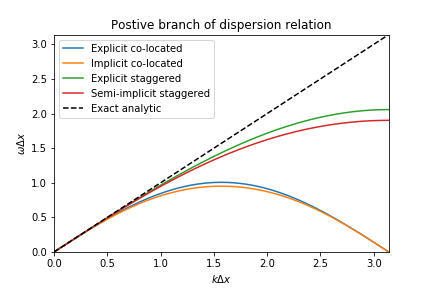
\includegraphics[width=0.7\textwidth]{dispersion_relations.png}
	\caption{Postive branch of dispersion relation $\omega$ for analytic solution and numerical schemes. Note that as in \cite{MPE textbook}, we have used $c=0.4$ and $\sqrt{gH} = 1$.} \label{dispersionfigure}
\end{figure}

\section{Methodology to test Numerical Methods}
In order to test the properties of the numerical methods outlined in the above section we have devised a series of tests on a variety of initial conditions.

\renewcommand\theContinuedFloat{\alph{ContinuedFloat}}
\begin{figure}
	\begin{minipage}{.5\textwidth}
		\ContinuedFloat*
		%\centering
		\captionsetup{width=0.9\textwidth}
		\captionsetup{justification=centering}
		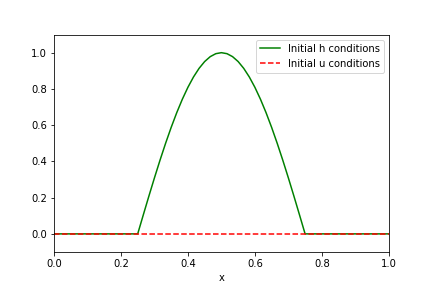
\includegraphics[width=\textwidth]{initial_condition_cosbell.png}
		\caption{\label{initialconditioncosbell}Initial condition such that $u$ is zero everywhere and $h$ has a bump in the centre with zero either side (hereafter referred to as cosbell)} 
	\end{minipage}
	\begin{minipage}{.5\textwidth}
		\ContinuedFloat
		%\centering
		\captionsetup{width=0.9\textwidth}
		\captionsetup{justification=centering}
		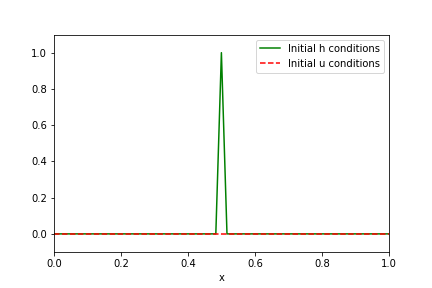
\includegraphics[width=\textwidth]{initial_condition_spike.png}
		\caption{\label{initialconditionspike}Initial condition such that $u$ is zero everywhere and $h$ is zero everywhere apart from one point at the centre where it is one} 
	\end{minipage}
	\begin{minipage}{.5\textwidth}
			\ContinuedFloat
			%\centering
			\captionsetup{width=0.9\textwidth}
			\captionsetup{justification=centering}
			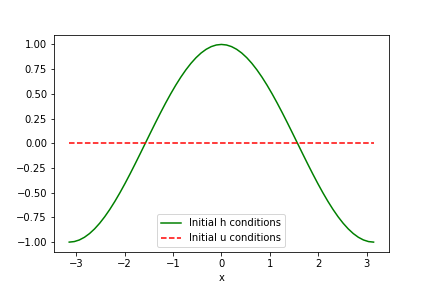
\includegraphics[width=\textwidth]{initial_condition_cos.png}
			\caption{\label{initialconditioncos}Initial condition such that $u$ is zero everywhere and $h$ is $\cos(x)$}
		\end{minipage}
		\begin{minipage}{.5\textwidth}
		\ContinuedFloat
		%\centering
		\captionsetup{width=0.9\textwidth}
		\captionsetup{justification=centering}
		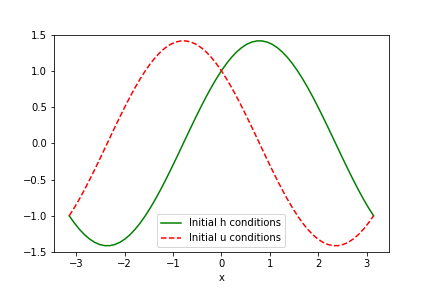
\includegraphics[width=\textwidth]{initial_condition_cossin.png}
		\caption{\label{initialconditioncossin}Initial condition such that $u$ is $\cos(x) - \sin(x)$ and $h$ is $\cos(x) + \sin(x)$}
	\end{minipage}
\end{figure}

\subsection{Test 1}
To begin with, we attempt to solve the shallow water equations using a simple initial condition (shown in Figure \ref{initialconditioncosbell}) with the co-located forward-backward explicit scheme.

\subsection{Test 2}
We found using Von-Neumann stability analysis that the co-located forward-backward explicit scheme is unstable for courant numbers higher than 2. Therefore this test will determine if this is in fact the case.

\subsection{Test 3}
We found using Von-Neumann stability analysis that the co-located forward-backward implicit scheme is stable for all courant numbers. Therefore this test will determine if this is in fact the case.

\subsection{Test 4}
When looking at the dispersion relation for the co-located grid it seems that the results produced by the scheme may be unphysical. We test this hypothesis by taking a different less smooth initial condition (shown in Figure \ref{initialconditionspike}) and plotting the solutions of $u$ and $h$ at multiple time steps for the co-located forward-backward explicit scheme and the co-located forward-backward implicit scheme.

\subsection{Test 5}
Our analysis of the dispersion relations suggests that on a staggered grid the solutions for $u$ and $h$ should be more physical. Therefore we repeat Test 4 with the same initial conditions (shown in Figure \ref{initialconditionspike}), but instead using the staggered explicit scheme.

\subsection{Test 6}
In the previous tests, the comparisons have been about the properties of the schemes themselves. If the initial condition shown in Figure \ref{initialconditioncos} is chosen it is possible to find an analytic solution of the shallow water equations
\begin{equation}\label{uanalytic}
u = \sin(x)\sin(t)
\end{equation}
\begin{equation}\label{hanalytic}
h = \cos(x)\cos(t).
\end{equation}
If we choose the interval $[-\pi, \pi]$ then these solutions are periodic.

This test will look at the solution errors between the solutions produced by the numerical schemes and the analytic solution. 

\subsection{Test 7}

In this test we would like to see if the orders of accuracy with respect to $\Delta x$ and $\Delta t$ found by Taylor expansion analysis in section \ref{numericalmethodssection} are correct. 
Also to further test that our numerical schemes give the correct solution to shallow water equation, we have chosen to compare to another analytical solution of the shallow water equations: 
\begin{eqnarray}
u = (\cos(x) - \sin(x))(\cos(t) - \sin(t))\\
h = (\cos(x) + \sin(x))(\cos(t) + \sin(t))
\end{eqnarray}
which corresponds to the initial condition shown in Figure \ref{initialconditioncossin}.

\subsection{Test 8}
Finally we compare the computational cost of the four schemes, by comparing the time it takes for each scheme to run, starting from the same initial condition (shown in Figure \ref{initialconditioncos}) and with the same number of time steps and space steps.

We would expect the co-located explicit and the staggered explicit schemes to take the same amount of time as the number of floating point operations per iteration of each scheme is the same. 

The implicit schemes have a higher computational cost than the explicit schemes as they involve one inversion of a matrix (O($n^{3}$) floating point operations for an $n \times n$ matrix) and at each iteration to find $u^{m}$ or $h^{m}$ a matrix-vector multiplication (O($n^{2}$) floating point operations for an $n \times n$ matrix). 

The staggered semi-implicit scheme has the highest computational cost, as constructing $b_{i}$ in the $A_{ij}x_{j} = b_{i}$ matrix equation involves nine floating point operations compared to three floating point operations to construct $b_{i}$ in the co-located implicit scheme.

\section{Results}\label{results section}
For all the following results, unless otherwise explicitily stated, assume the domain used was $0 \leq x \leq 1$ and that the following parameters were used:

\begin{eqnarray}
c & = & 0.1\\
H & = & 1\\
g & = & 1\\
nx & = & 60\\
nt & = & 100
\end{eqnarray}
where $c$ is the courant number, $H$ is the average fluid depth, $g$ is the gravitational acceleration constant, $nx$ is the number of space-steps in the meshgrid and $nt$ is the number of time-steps.
\subsection{Test 1}
\begin{figure} [H]
	\begin{minipage}{.5\textwidth}
		\ContinuedFloat*
		%\centering
		\captionsetup{width=0.9\textwidth}
		\captionsetup{justification=centering}
		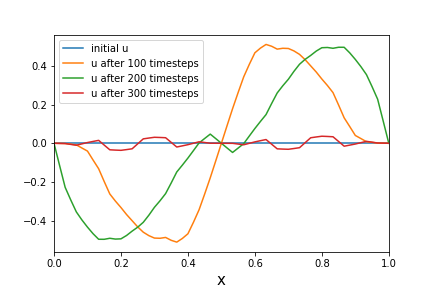
\includegraphics[width=\textwidth]{velocity_colocated_explicit_cosbell.png}
		\caption{\label{velocity_colocated_explicit_cosbell} Velocity at different timesteps using the co-located explicit method using the initial condition $u$ equals $0$ and $h$ is a cosbell (as shown in Figure \ref{initialconditioncosbell}).} 
	\end{minipage}
	\begin{minipage}{.5\textwidth}
		\ContinuedFloat
		%\centering
		\captionsetup{width=0.9\textwidth}
		\captionsetup{justification=centering}
		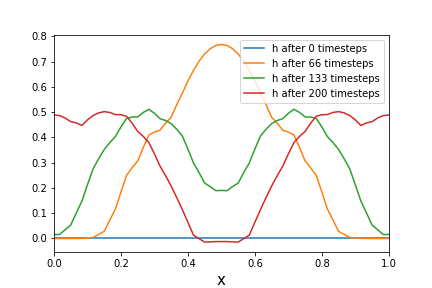
\includegraphics[width=\textwidth]{height_colocated_explicit_cosbell.png}
		\caption{\label{height_colocated_explicit_cosbell}    Height at different timesteps using the co-located explicit method using the initial condition $u$ equals $0$ and $h$ is a cosbell (as shown in Figure \ref{initialconditioncosbell}).} 
	\end{minipage}
\end{figure}
In this test we have successfully shown that we can use the co-located explicit schemes to solve the shallow water equations. These solutions seem to make physical sense as in Figure \ref{height_colocated_explicit_cosbell} we can see fluid falling from a peak and then separating over time as we would expect.

\subsection{Test 2}\label{sectiontest2}

\begin{figure} [H]
	\begin{minipage}{.5\textwidth}
		\ContinuedFloat*
		%\centering
		\captionsetup{width=0.9\textwidth}
		\captionsetup{justification=centering}
		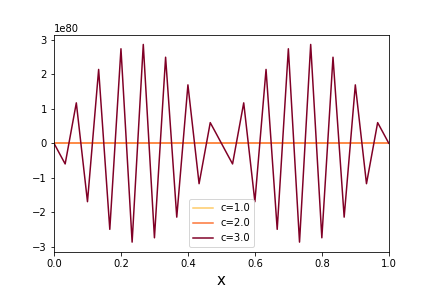
\includegraphics[width=\textwidth]{velocity_varying_courant_explicit.png}
		\caption{\label{velocity_varying_courant_explicit} Velocity for varying courant numbers for the co-located explicit method} 
	\end{minipage}
	\begin{minipage}{.5\textwidth}
		\ContinuedFloat
		%\centering
		\captionsetup{width=0.9\textwidth}
		\captionsetup{justification=centering}
		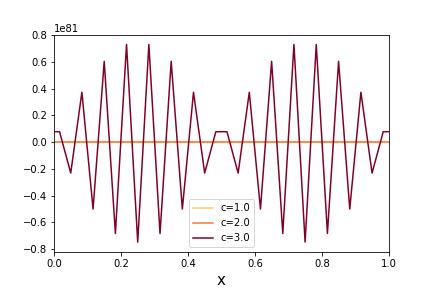
\includegraphics[width=\textwidth]{height_varying_courant_explicit.png}
		\caption{\label{height_varying_courant_explicit} Height for varying courant numbers for the co-located explicit method} 
	\end{minipage}
\end{figure}

Figure \ref{velocity_varying_courant_explicit} and Figure \ref{height_varying_courant_explicit} show that for large courant numbers, $u$ and $h$ are very unstable reaching values of an order of magnitude of $10^{80}$. This is as we expected from the Von-Neumann stability analysis.

\subsection{Test 3}

\begin{figure} [H]
	\begin{minipage}{.5\textwidth}
		\ContinuedFloat*
		%\centering
		\captionsetup{width=0.9\textwidth}
		\captionsetup{justification=centering}
		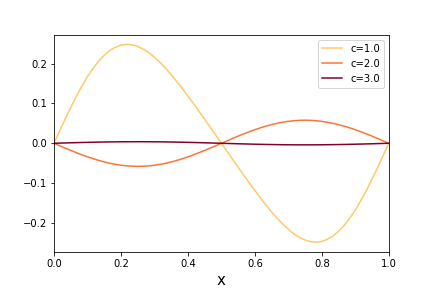
\includegraphics[width=\textwidth]{velocity_varying_courant_implicit.png}
		\caption{\label{velocity_varying_courant_implicit} Velocity for varying courant numbers for the co-located implicit method} 
	\end{minipage}
	\begin{minipage}{.5\textwidth}
		\ContinuedFloat
		%\centering
		\captionsetup{width=0.9\textwidth}
		\captionsetup{justification=centering}
		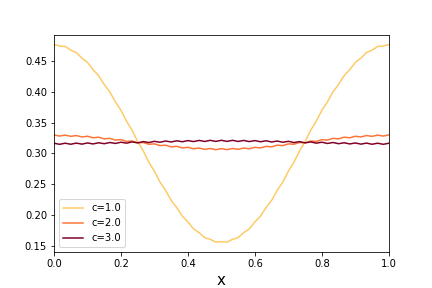
\includegraphics[width=\textwidth]{height_varying_courant_implicit.png}
		\caption{\label{height_varying_courant_implicit} Height for varying courant numbers for the co-located implicit method} 
	\end{minipage}
\end{figure}

By contrast with the co-located explicit method tested in test 2 (\ref{sectiontest2}), when using the co-located implicit method, Figure \ref{velocity_varying_courant_implicit} and Figure \ref{height_varying_courant_implicit} show that for large courant numbers, $u$ and $h$ remain stable. This is as we expected from the Von-Neumann stability analysis.

\subsection{Test 4}\label{subsectiontest4}

Note for this test we have used $nx = 20$ and $nt = 10$ (all other parameters remain the same).

\begin{figure} [H]
	\begin{minipage}{.5\textwidth}
		\ContinuedFloat*
		%\centering
		\captionsetup{width=0.9\textwidth}
		\captionsetup{justification=centering}
		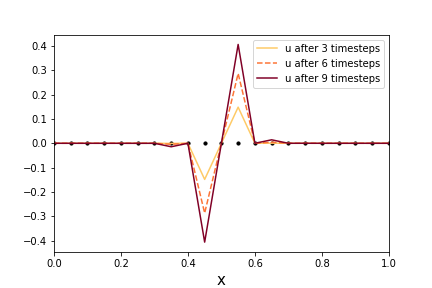
\includegraphics[width=\textwidth]{velocity_colocated_explicit_spike.png}
		\caption{\label{velocity_colocated_explicit_spike} Velocity at different timesteps using the co-located explicit method using the initial condition $u$ equals 0 and $h$ is a spike (as shown in Figure \ref{initialconditionspike}).} 
	\end{minipage}
	\begin{minipage}{.5\textwidth}
		\ContinuedFloat
		%\centering
		\captionsetup{width=0.9\textwidth}
		\captionsetup{justification=centering}
		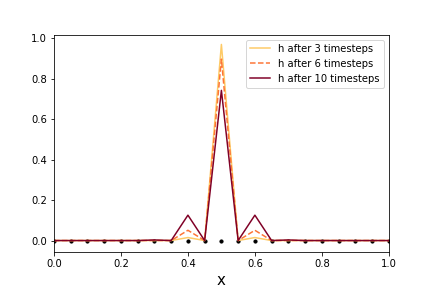
\includegraphics[width=\textwidth]{height_colocated_explicit_spike.png}
		\caption{\label{height_colocated_explicit_spike} Height at different timesteps using the co-located explicit method using the initial condition $u$ equals 0 and $h$ is a spike (as shown in Figure \ref{initialconditionspike}).} 
	\end{minipage}
\end{figure}

\begin{figure} [H]
	\begin{minipage}{.5\textwidth}
		\ContinuedFloat*
		%\centering
		\captionsetup{width=0.9\textwidth}
		\captionsetup{justification=centering}
		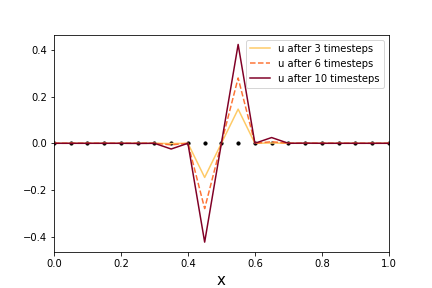
\includegraphics[width=\textwidth]{velocity_colocated_implicit_spike.png}
		\caption{\label{velocity_colocated_implicit_spike} Velocity at different timesteps using the co-located implicit method using the initial condition $u$ equals 0 and $h$ is a spike (as shown in Figure \ref{initialconditionspike}).} 
	\end{minipage}
	\begin{minipage}{.5\textwidth}
		\ContinuedFloat
		%\centering
		\captionsetup{width=0.9\textwidth}
		\captionsetup{justification=centering}
		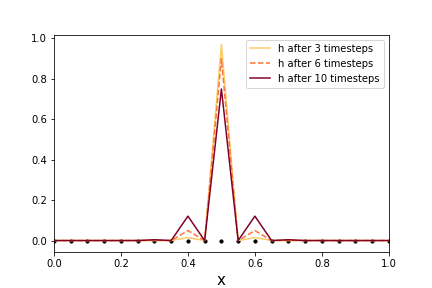
\includegraphics[width=\textwidth]{height_colocated_implicit_spike.png}
		\caption{\label{height_colocated_implicit_spike} Height at different timesteps using the co-located implicit method using the initial condition $u$ equals 0 and $h$ is a spike (as shown in Figure \ref{initialconditionspike}).} 
	\end{minipage}
\end{figure}

As expected the results shown in Figures \ref{velocity_colocated_explicit_spike}, \ref{height_colocated_explicit_spike}, \ref{velocity_colocated_implicit_spike} and \ref{height_colocated_implicit_spike} are unphysical. The fluid does spread out but it does not go to the next meshpoint, instead skipping this meshpoint out and moving to the next meshpoint along. In Figure \ref{height_colocated_explicit_spike} and {\ref{height_colocated_implicit_spike}, we see that the two points around the central grid point (hereafter referred to as $x_{m}$) never have any height so the fluid passes from $x_{m}$ to $x_{m-2}$ and $x_{m+ 2}$ without passing through $x_{m-1}$ and $x_{m+1}$ which is clearly unphysical. Similarly in Figure \ref{velocity_colocated_explicit_spike} and \ref{velocity_colocated_implicit_spike} there is never any velocity at the gridpoints $x_{m-2}$ and $x_{m+2}$ which is again unphysical. 
	
Therefore our hypothesis that the results are unphysical is true.

\subsection{Test 5}
Note for this test we have used $nx = 20$ and $nt = 10$ (all other parameters remain the same).
\begin{figure} [H]
	\begin{minipage}{.5\textwidth}
		\ContinuedFloat*
		%\centering
		\captionsetup{width=0.9\textwidth}
		\captionsetup{justification=centering}
		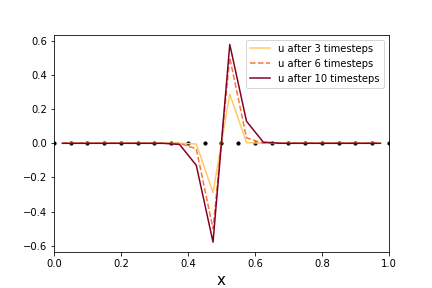
\includegraphics[width=\textwidth]{velocity_staggered_explicit_spike.png}
		\caption{\label{velocity_staggered_explicit_spike} Velocity at different timesteps using the staggered explicit method using the initial condition $u$ equals 0 and $h$ is a spike (as shown in Figure \ref{initialconditionspike}).} 
	\end{minipage}
	\begin{minipage}{.5\textwidth}
		\ContinuedFloat
		%\centering
		\captionsetup{width=0.9\textwidth}
		\captionsetup{justification=centering}
		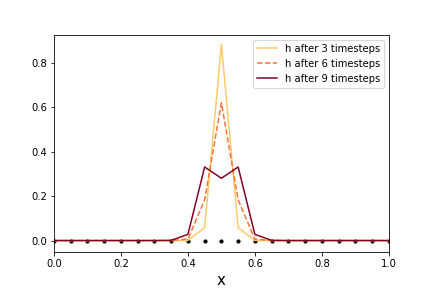
\includegraphics[width=\textwidth]{height_staggered_explicit_spike.png}
		\caption{\label{height_staggered_explicit_spike} Height at different timesteps using the staggered explicit method using the initial condition $u$ equals 0 and $h$ is a spike (as shown in Figure \ref{initialconditionspike}).} 
	\end{minipage}
\end{figure}

As expected in contrast to the results in the previous test (\ref{subsectiontest4}), the staggered scheme produces physical results for this initial condition. Figure \ref{height_staggered_explicit_spike} shows that the height spreads out evenly using all grid points. Figure \ref{velocity_staggered_explicit_spike} shows further that the velocity is non-zero at the gridpoints where the wave has so far propagated as we would expect in a physically realistic system.

\subsection{Test 6}

Note for this test we have used $c = 1$, $nx = 1000$, $nt = 1000$ and the domain $=\pi\leq x \leq \pi$.
\begin{figure} [H]
	\begin{minipage}{.5\textwidth}
		\ContinuedFloat*
		%\centering
		\captionsetup{width=0.9\textwidth}
		\captionsetup{justification=centering}
		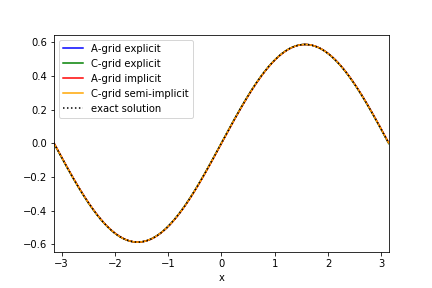
\includegraphics[width=\textwidth]{comparison_with_exact_u.png}
		\caption{\label{exact velocity} Velocity, $u$, for the initial condition where $u$ is 0 everywhere and $h$ is $\cos(x)$ (as shown in Figure \ref{initialconditioncos}). } 
	\end{minipage}
	\begin{minipage}{.5\textwidth}
		\ContinuedFloat
		%\centering
		\captionsetup{width=0.9\textwidth}
		\captionsetup{justification=centering}
		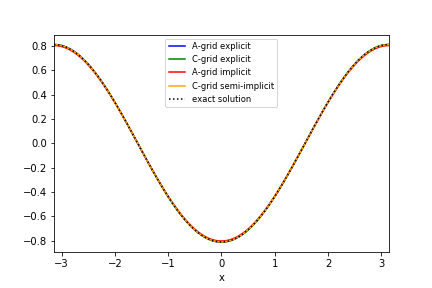
\includegraphics[width=\textwidth]{comparison_with_exact_h.png}
		\caption{\label{exact height} Height, $h$, for the initial condition where $u$ is 0 everywhere and $h$ is $\cos(x)$ (as shown in Figure \ref{initialconditioncos}).} 
	\end{minipage}
\end{figure}
Figures \ref{exact velocity} and \ref{exact height} show that for the smooth initial condition $u= 0$ and $h= \cos(x)$, all the numerical schemes approximate very closely to the analytical solution. 

To distinguish which method is better, we have calculated the L2 error norms of the schemes in Table \ref{errortable}. These show that the staggered semi-implicit method is the most accurate, as expected as it is second order in time and space whereas the other schemes are first order in time and second order in space. Unexpectedly the co-located implicit scheme is more inaccurate than the other schemes for $u$. This may be because of cumulative errors when inverting and multiplying the matrix used in the scheme.

%\begin{figure} [H]
%	\begin{minipage}{.5\textwidth}
%		\ContinuedFloat*
%		%\centering
%		\captionsetup{width=0.9\textwidth}
%		\captionsetup{justification=centering}
%		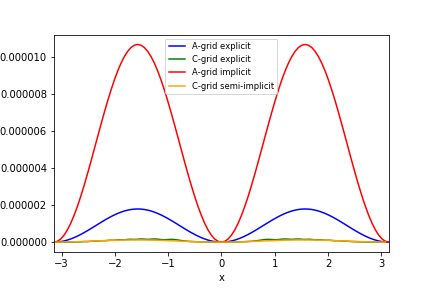
\includegraphics[width=\textwidth]{error_in_u.png}
%		\caption{\label{error_velocity} Error in velocity, for the initial condition where $u$ is 0 everywhere and $h$ is $\cos(x)$ (as shown in Figure \ref{initialconditioncos}). Note here we have used $c = 1$, $nx = 1000$, $nt = 1000$ and the domain $=\pi\leq x \leq \pi$.} 
%	\end{minipage}
%	\begin{minipage}{.5\textwidth}
%		\ContinuedFloat
		%\centering
%		\captionsetup{width=0.9\textwidth}
%		\captionsetup{justification=centering}
%		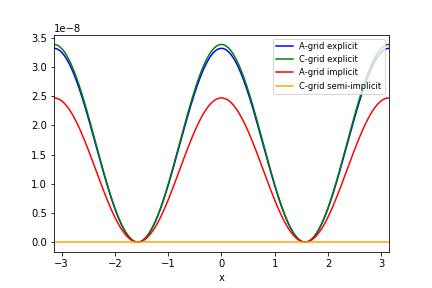
\includegraphics[width=\textwidth]{error_in_h.png}
%		\caption{\label{error_height} Error in height, for the initial condition where $u$ is 0 everywhere and $h$ is $\cos(x)$ (as shown in Figure \ref{initialconditioncos}). Note here we have used $c = 1$, $nx = 1000$, $nt = 1000$ and the domain $=\pi\leq x \leq \pi$.} 
%	\end{minipage}
%\end{figure}



\begin{table}[H]
	\centering
	\begin{tabular}{|c | c| c|} 
		\hline
		\textbf{Numerical Scheme} & \textbf{Error in u} & \textbf{Error in h}  \\
		\hline
		Co-located Explicit & $7.4 \times 10^{-5}$ & 0.0041\\ 
		\hline
		Staggered Explicit &  $2.0 \times 10^{-5}$ & 0.0041\\
		\hline
		Co-located  Implicit & 0.0027 & 0.0035 \\
		\hline
		Staggered Semi-implicit & $1.9 \times 10^{-5}$ & $1.39\times 10 ^{-5}$ \\
		\hline
	\end{tabular}
	\caption{Error L2 norms for all 4 numerical schemes}
	\label{errortable}
\end{table}

\subsection{Test 7}
Note for this test we have used $c = 0.1$ and varying $nx$ and $nt$ (to find the relationship between $\Delta x$, $\Delta t$ and the error) on the domain $-\pi \leq x \leq \pi$.
\begin{figure} [H]
	\begin{minipage}{.5\textwidth}
	\ContinuedFloat*
	%\centering
	\captionsetup{width=0.9\textwidth}
	\captionsetup{justification=centering}
	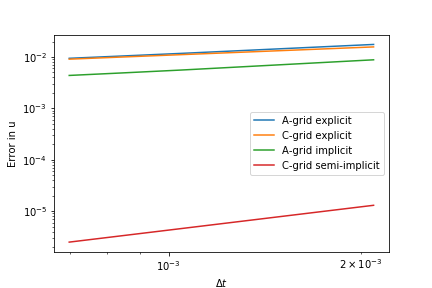
\includegraphics[width=\textwidth]{uerror_compared_dt_cossin.png}
	\caption{\label{uerrorcossindt}Log plot for the solution error of $u$ vs $\Delta t$ for the initial condition $u = \cos(x) - \sin(x)$ and $h = \cos(x) + \sin(x)$ (as shown in Figure \ref{initialconditioncossin})} 
\end{minipage}
\begin{minipage}{.5\textwidth}
	\ContinuedFloat
	%\centering
	\captionsetup{width=0.9\textwidth}
	\captionsetup{justification=centering}
	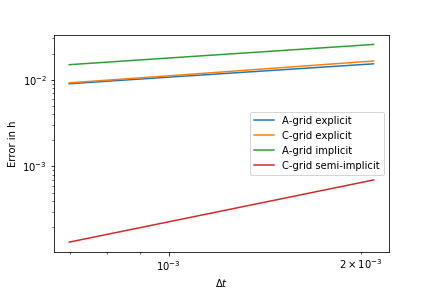
\includegraphics[width=\textwidth]{herror_compared_dt_cossin.png}
	\caption{\label{herrorcossindt}Log plot for the solution error of $h$ vs $\Delta t$ for the initial condition $u = \cos(x) - \sin(x)$ and $h = \cos(x) + \sin(x)$ (as shown in Figure \ref{initialconditioncossin})} 
\end{minipage}
	\begin{minipage}{.5\textwidth}
	\ContinuedFloat
	%\centering
	\captionsetup{width=0.9\textwidth}
	\captionsetup{justification=centering}
	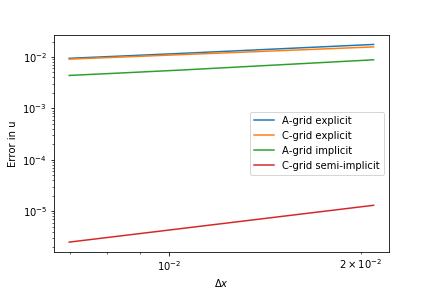
\includegraphics[width=\textwidth]{uerror_compared_dx_cossin.png}
	\caption{\label{uerrorcossindx}Log plot for the solution error of $u$ vs $\Delta x$ for the initial condition $u = \cos(x) - \sin(x)$ and $h = \cos(x) + \sin(x)$ (as shown in Figure \ref{initialconditioncossin})} 
\end{minipage}
	\begin{minipage}{.5\textwidth}
	\ContinuedFloat
	%\centering
	\captionsetup{width=0.9\textwidth}
	\captionsetup{justification=centering}
	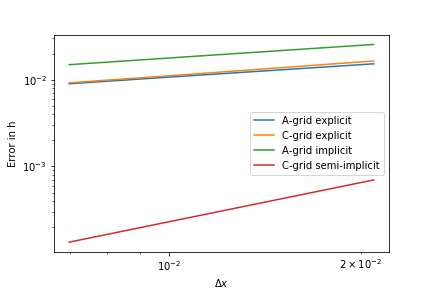
\includegraphics[width=\textwidth]{herror_compared_dx_cossin.png}
	\caption{\label{herrorcossindx}Log plot for the solution error of $h$ vs $\Delta x$ for the initial condition $u = \cos(x) - \sin(x)$ and $h = \cos(x) + \sin(x)$ (as shown in Figure \ref{initialconditioncossin})} 
\end{minipage}
\end{figure}
We see in Figures \ref{uerrorcossindt} - \ref{herrorcossindx} that the error plotted against $\Delta x$ and the error plotted against $\Delta t$ is the same. This is because as we are keeping the courant number, $c$, constant and the number of time steps, $nt$, and number of space steps, $nx$, constant, it is impossible to vary $\Delta x$ without varying $\Delta t$. We also see that as before in Test 6 the error in the semi-implicit method is much lower than the error for the other methods. In contrast to Test 6 the implicit method has the same order of accuracy as the co-located explicit and staggered explicit methods, as we would expect.

Table \ref{gradient} contains the gradient of the lines plotted in Figures \ref{uerrorcossindt} - \ref{herrorcossindx}. We would expect the gradient of the error vs. $\Delta x$ to be 2 for all schemes as they are all second order accurate in space. We would expect the error vs. $\Delta t$ to be 1 for all schemes apart from the staggered semi-implicit scheme for which it should be 2, because all the schemes are first order in time apart from the staggered semi-implicit scheme which is second order in time. However this is not what Table \ref{gradient} shows. One of the reasons may be because the $\Delta x$ and $\Delta t$ errors are being considered together so table \ref{gradient} contains cumulative orders of accuracy. Another may be that the higher order $\Delta x$ and $\Delta t$ terms are affecting the gradient. 

Our results do still show that the staggered semi-implicit method does have a higher order of accuracy than the other schemes which is as expected.

\begin{table}[H]
	\centering
	\begin{tabular}{|c | c| c| c| c|} 
		\hline
		\textbf{Numerical Scheme} & $u$ error vs $\Delta x$ &  $u$ error vs $\Delta t$ & $h$ error vs $\Delta x$ & $h$ error vs $\Delta t$\\
		\hline
		Co-located Explicit & 0.57 & 0.57 & 0.48 & 0.48\\ 
		\hline
		Staggered Explicit & 0.50 & 0.50 & 0.53 & 0.53 \\
		\hline
		Co-located Implicit & 0.64 & 0.64 & 0.49 & 0.49 \\
		\hline
		Staggered Semi-implicit & 1.50 & 1.50 & 1.50 & 1.50\\
		\hline
	\end{tabular}
	\caption{Gradient of functions shown in Figures \ref{uerrorcossindt} - \ref{herrorcossindx} ie. log of meshgrid vs log of error for the initial condition $u = \cos(x) - \sin(x)$ and $h = \cos(x) + \sin(x)$}
	\label{gradient}
\end{table}


%Analytical solution is $u = \sin(x)\sin(t)$ and $h = \cos(x)\cos(t)$
%\begin{table}[H]
%	\centering
%	\begin{tabular}{|c | c| c| c| c|} 
%		\hline
%		\textbf{Numerical Scheme} & $u$ error vs $\Delta x$ &  $u$ error vs $\Delta t$ & $h$ error vs $\Delta x$ & $h$ error vs $\Delta t$\\
%		\hline
%		Co-located Explicit & 1.50 & 1.50 &  0.45& 0.45\\ 
%		\hline
%		Staggered Explicit & 1.50 & 1.50 & 0.49 & 0.49 \\
%		\hline
%		Co-located Implicit & 0.52 & 0.52 & 0.42 & 0.42 \\
%		\hline
%		Staggered Semi-implicit & 1.50 & 1.50 & 1.50 & 1.50\\
%		\hline
%	\end{tabular}
%	\caption{}
%	\label{}
%\end{table}

\subsection{Test 8}
Note for this test the number of space steps is 1000 and number of time steps is 1000.
\begin{table}[H]
	\centering
	\begin{tabular}{|c | c|} 
		\hline
		\textbf{Numerical Scheme} & \textbf{Time (3sf)}  \\
		\hline
		Co-located Explicit & 2.07 s \\ 
		\hline
	    Staggered Explicit & 1.96 s \\
		\hline
		Co-located  Implicit & 3.23 s \\
		\hline
		Staggered Semi-implicit & 84.5 s \\
		\hline
	\end{tabular}
\caption{Time taken for each numerical scheme to run for the initial condition that $h$ is $\cos(x)$ and $u$ is $0$ (as shown in Figure \ref{initialconditioncos}).}
\label{timingtable}
\end{table}

Table \ref{timingtable} shows as expected that the staggered semi-implict scheme takes the longest of the four schemes. The co-located explicit and staggered explicit schemes take a similar amount of time as expected as the number of floating point operations per iteration is the same for both schemes. Again as expected he co-located implicit scheme takes slightly longer than the explicit schemes but not as long as the staggered semi-implicit scheme. This is because the construction of the vector $b$ in the matrix equation is simpler for the co-located implicit scheme than for the staggered semi-implicit scheme.

\newpage

\section{Conclusions}

From the results listed in Section \ref{results section}, we can conclude the following:

\begin{itemize}
	\item When working with high courant numbers (e.g. if the meshgrid spacing is very fine so $\Delta x$ is small or if $H$ or $\Delta t$ are very large), it is better to choose implicit methods as they are stable for all courant numbers whereas explicit methods can have large instabilities (from Test 2 and Test 3)
	\item Staggered grids produce more physically realistic results than co-located grids for certain initial conditions (from Test 4 and Test 5)
	\item The semi-implicit staggered method is the most accurate of the 4 schemes (from Test 6 and Test 7)
	\item When working with small courant numbers, it is better to choose explicit methods as they are much less computationally expensive than implicit methods (from Test 8)
\end{itemize}


\begin{thebibliography}{9}
	\addcontentsline{toc}{part}{Bibliography}
	\bibitem{MPE textbook}
	Cotter, C. and Weller, H., (2018), \textquoteleft Numerical Methods\textquoteright, Ch.5 in Crisan, D (eds.), \textit{Mathematics of Planet Earth: a primer}, World Scientific Publishing Europe Ltd., London.
	\bibitem{semi-implicit}
	Casulli, V. and Cattani, E., (1994), \textquoteleft Stability, Accuracy and Efficiency of a Semi-Implicit Method for Three-Dimensional Shallow Water Flow\textquoteright, \textit{Computers Math. Applic}, \textbf{27(4)}, 99-112.
\end{thebibliography}
\end{document}